\chapter{Motivation}
\label{chap:motiviation}
\thispagestyle{fancy}

\section{Problem}
\label{sec:problem}

While doing their groceries, the majority of people are free to follow their own taste and purchase any food item without having to worry about putting their health at risk. However, a significant part of the Swiss population must take a closer look on the products they are about to buy: According to \citeauthor{AhaAllergies}, 30 percent of Switzerland's population asserts to be suffering from food allergies (\citeyear{AhaAllergies}) and 20 percent claim to be affected by at least one form of food intolerance (\citeyear{AhaIntolerances}).

Therefore, it is crucial that products sold in grocery stores are labeled adequately in order to prevent health risks, such as allergic reactions and intolerances to foods. According to Swiss law, 14 specific ingredients and all products derived therefrom are considered as potentially harmful and therefore have to be declared. These allergens must be displayed in "text or number", which can be complemented or even substituted by icons \citep{FoodLaw}.

Currently, most food manufactures use a text-only approach and follow a common best practice: if an entry in the list of ingredients contains a potential allergen or products derived therefrom, the text section in the entry which indicates the allergen is emphasized by capitalization or using a bold font (\cref{fig:label-ingredients}). Additionally, some food packages also carry an information box which summarizes all the contained allergens (\cref{fig:label-allergens}), however, it is not very common in practice.

\begin{figure}[ht]
     \centering
     
     \begin{subfigure}[b]{0.5\textwidth}
         \centering
         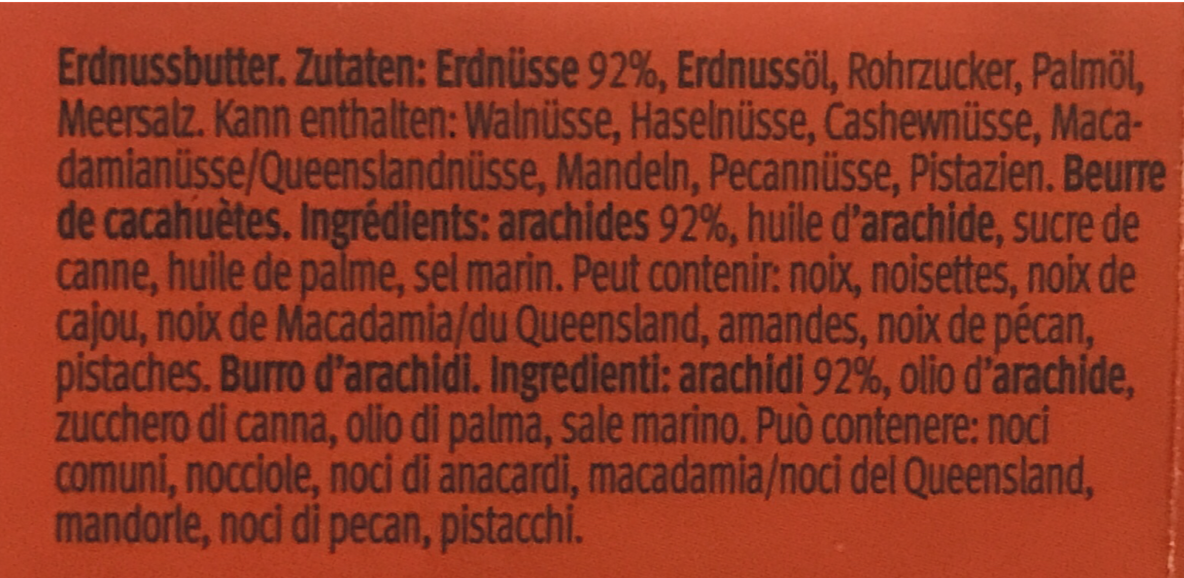
\includegraphics[width=\textwidth]{label-ingredients}
         \caption{Emphasised allergens}
         \label{fig:label-ingredients}
     \end{subfigure}
          \hfill
     \begin{subfigure}[b]{0.4\textwidth}
         \centering
         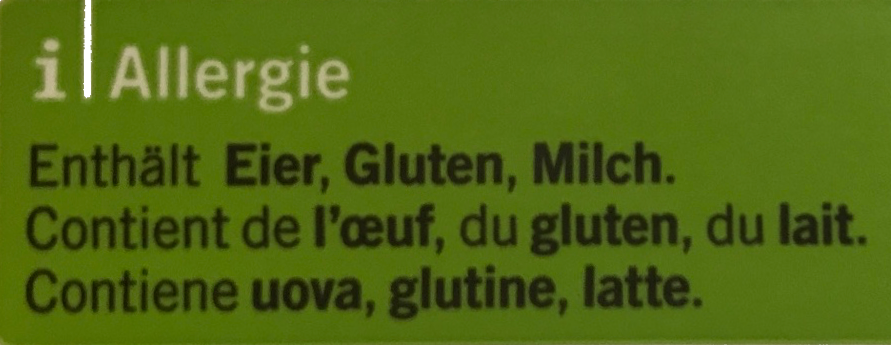
\includegraphics[width=\textwidth]{label-allergens}
         \caption{Listing of allergens}
         \label{fig:label-allergens}
     \end{subfigure}
        \caption{Presentation of contained allergens}
        \label{fig:labels}
\end{figure}

The trend towards text-only presentation inherently carries an increased danger of people not being able to identify a subjective critical ingredient due to language barriers. Switzerland has four official languages and the product information is mainly stated in German, French and Italian. 95 percent of the Swiss population at the age of 15 or older consider one of these language as their first language and thus are able to understand the information on the product package. However, five percent of the population or 376’000 permanent residents are presumably not able to understand the information in any of the three languages, hence that fraction of the population is left in the dark \citep{Languages}. It should also be noted that the visiting tourists possibly face difficulties as well while purchasing products which correspond to their allergy profile.


\section{Approach}

The aim of the project at hand is to develop a smartphone application called \emph{Allergy Scan} that enables a superior visualization of the allergens contained in food items. The main objective is to evaluate if there are any possible improvements to the current textual approach and if an application like Allergy Scan can be a superior solution to the existing problems.

The application requires the users to list their critical allergens and scan the bar code of the food item they are considering to purchase. Subsequently the users receive information about the food item’s allergen profile.

Each user is assigned to one of four test groups. The groups differ from one another in the way the allergens are displayed (tailoring) and visualized (visualization). After the user became familiar with the application through an intensive preoccupation with it, a feedback will be obtained. The user must rate several aspects of the app and its usage, such as to which extent the app facilitates the user’s dealing with food allergies.

Afterwards the collected data will be analyzed in the light of demographic criteria and usage behavior. In a next step the data within the different test groups will be aggregated to find out which combination of tailoring and visualization generates the best user satisfaction and thus should be examined in detail in further studies.